\chapter{Results} \label{ch:results}
Present results and comparisons to Adare et al.....

	\begin{figure}[h]
	  \centering
	  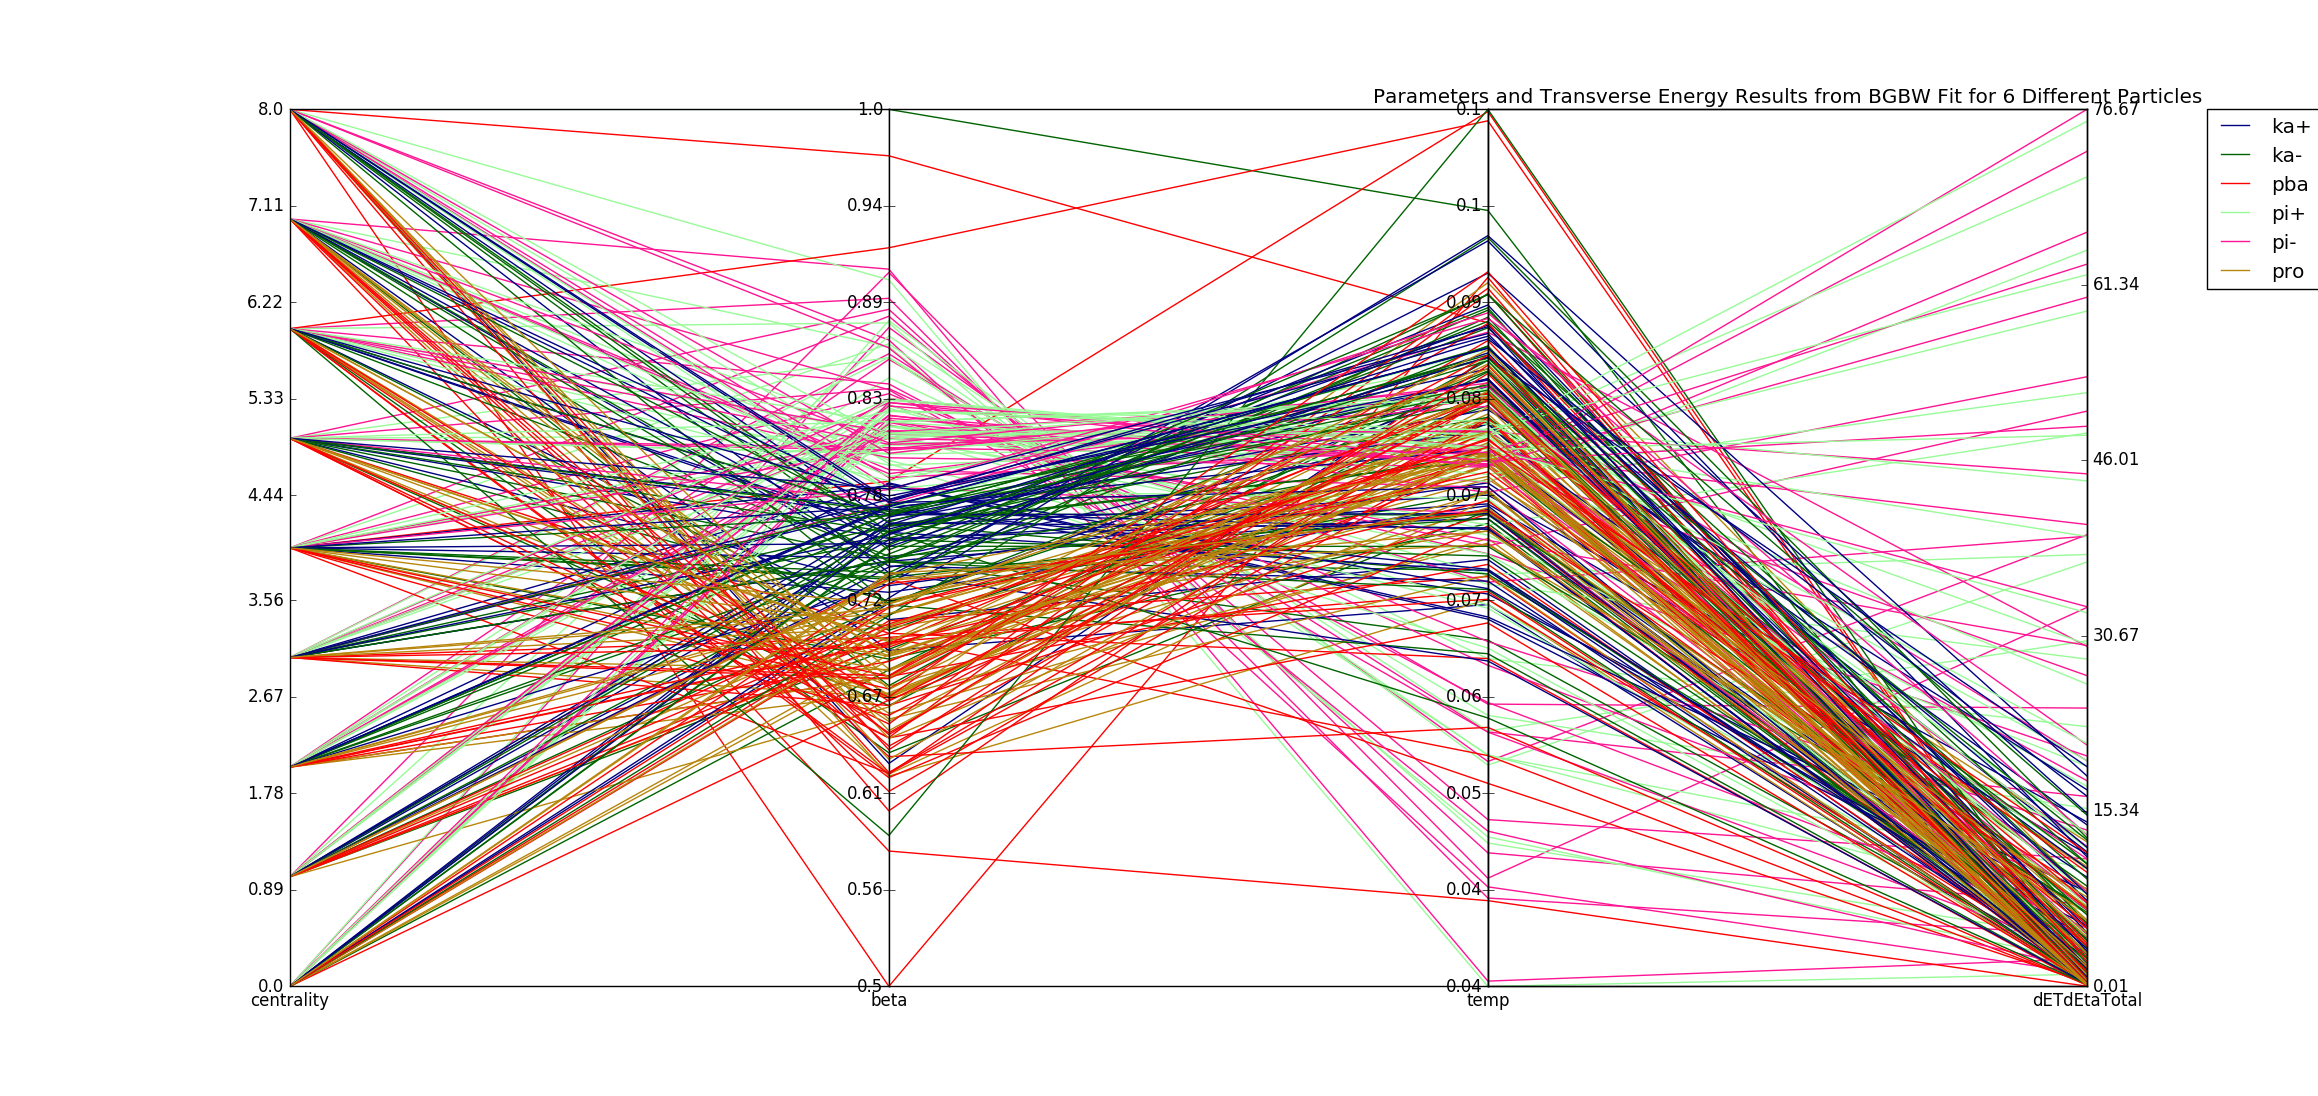
\includegraphics[width=6.5in]{figures/parallelCoordPlot_4Axes.png}
	  \caption{Parallel coordinates plot for 270 diffrent spectra relating 6 different identified particles (color-coded) to their respective collision centrality classes, good-fit parameters, and the transverse energy calculated using said parameters.}\label{fig:parallelCoord}
	\end{figure}
	
	\begin{figure}[h]
	  \centering
	  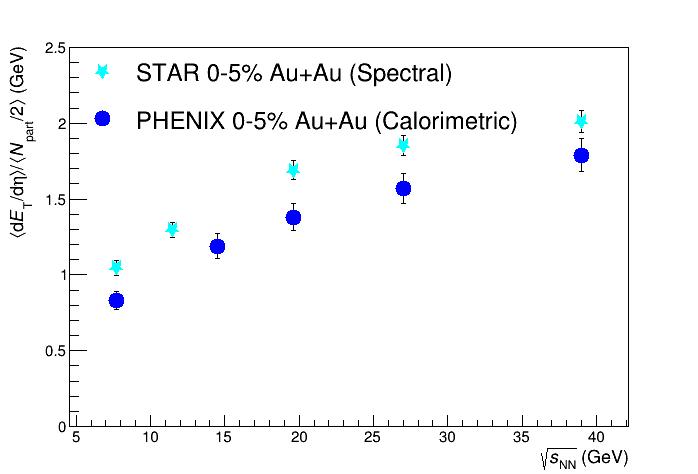
\includegraphics[width=4.5in]{figures/PHENIX_comparison2.png}
	  \caption{$\frac{dE_{T}}{d\eta}/0.5N_{part}$ for 0-5\% central collisions at midrapidity as a function of $\sqrt{s_{NN}}$. The PHENIX data are from \cite{PhysRevC.93.024901}. The error bars represent the total statistical and systematic uncertainties.}\label{fig:comparison}
	\end{figure}
	
	\begin{figure}[h]
	  \centering
	  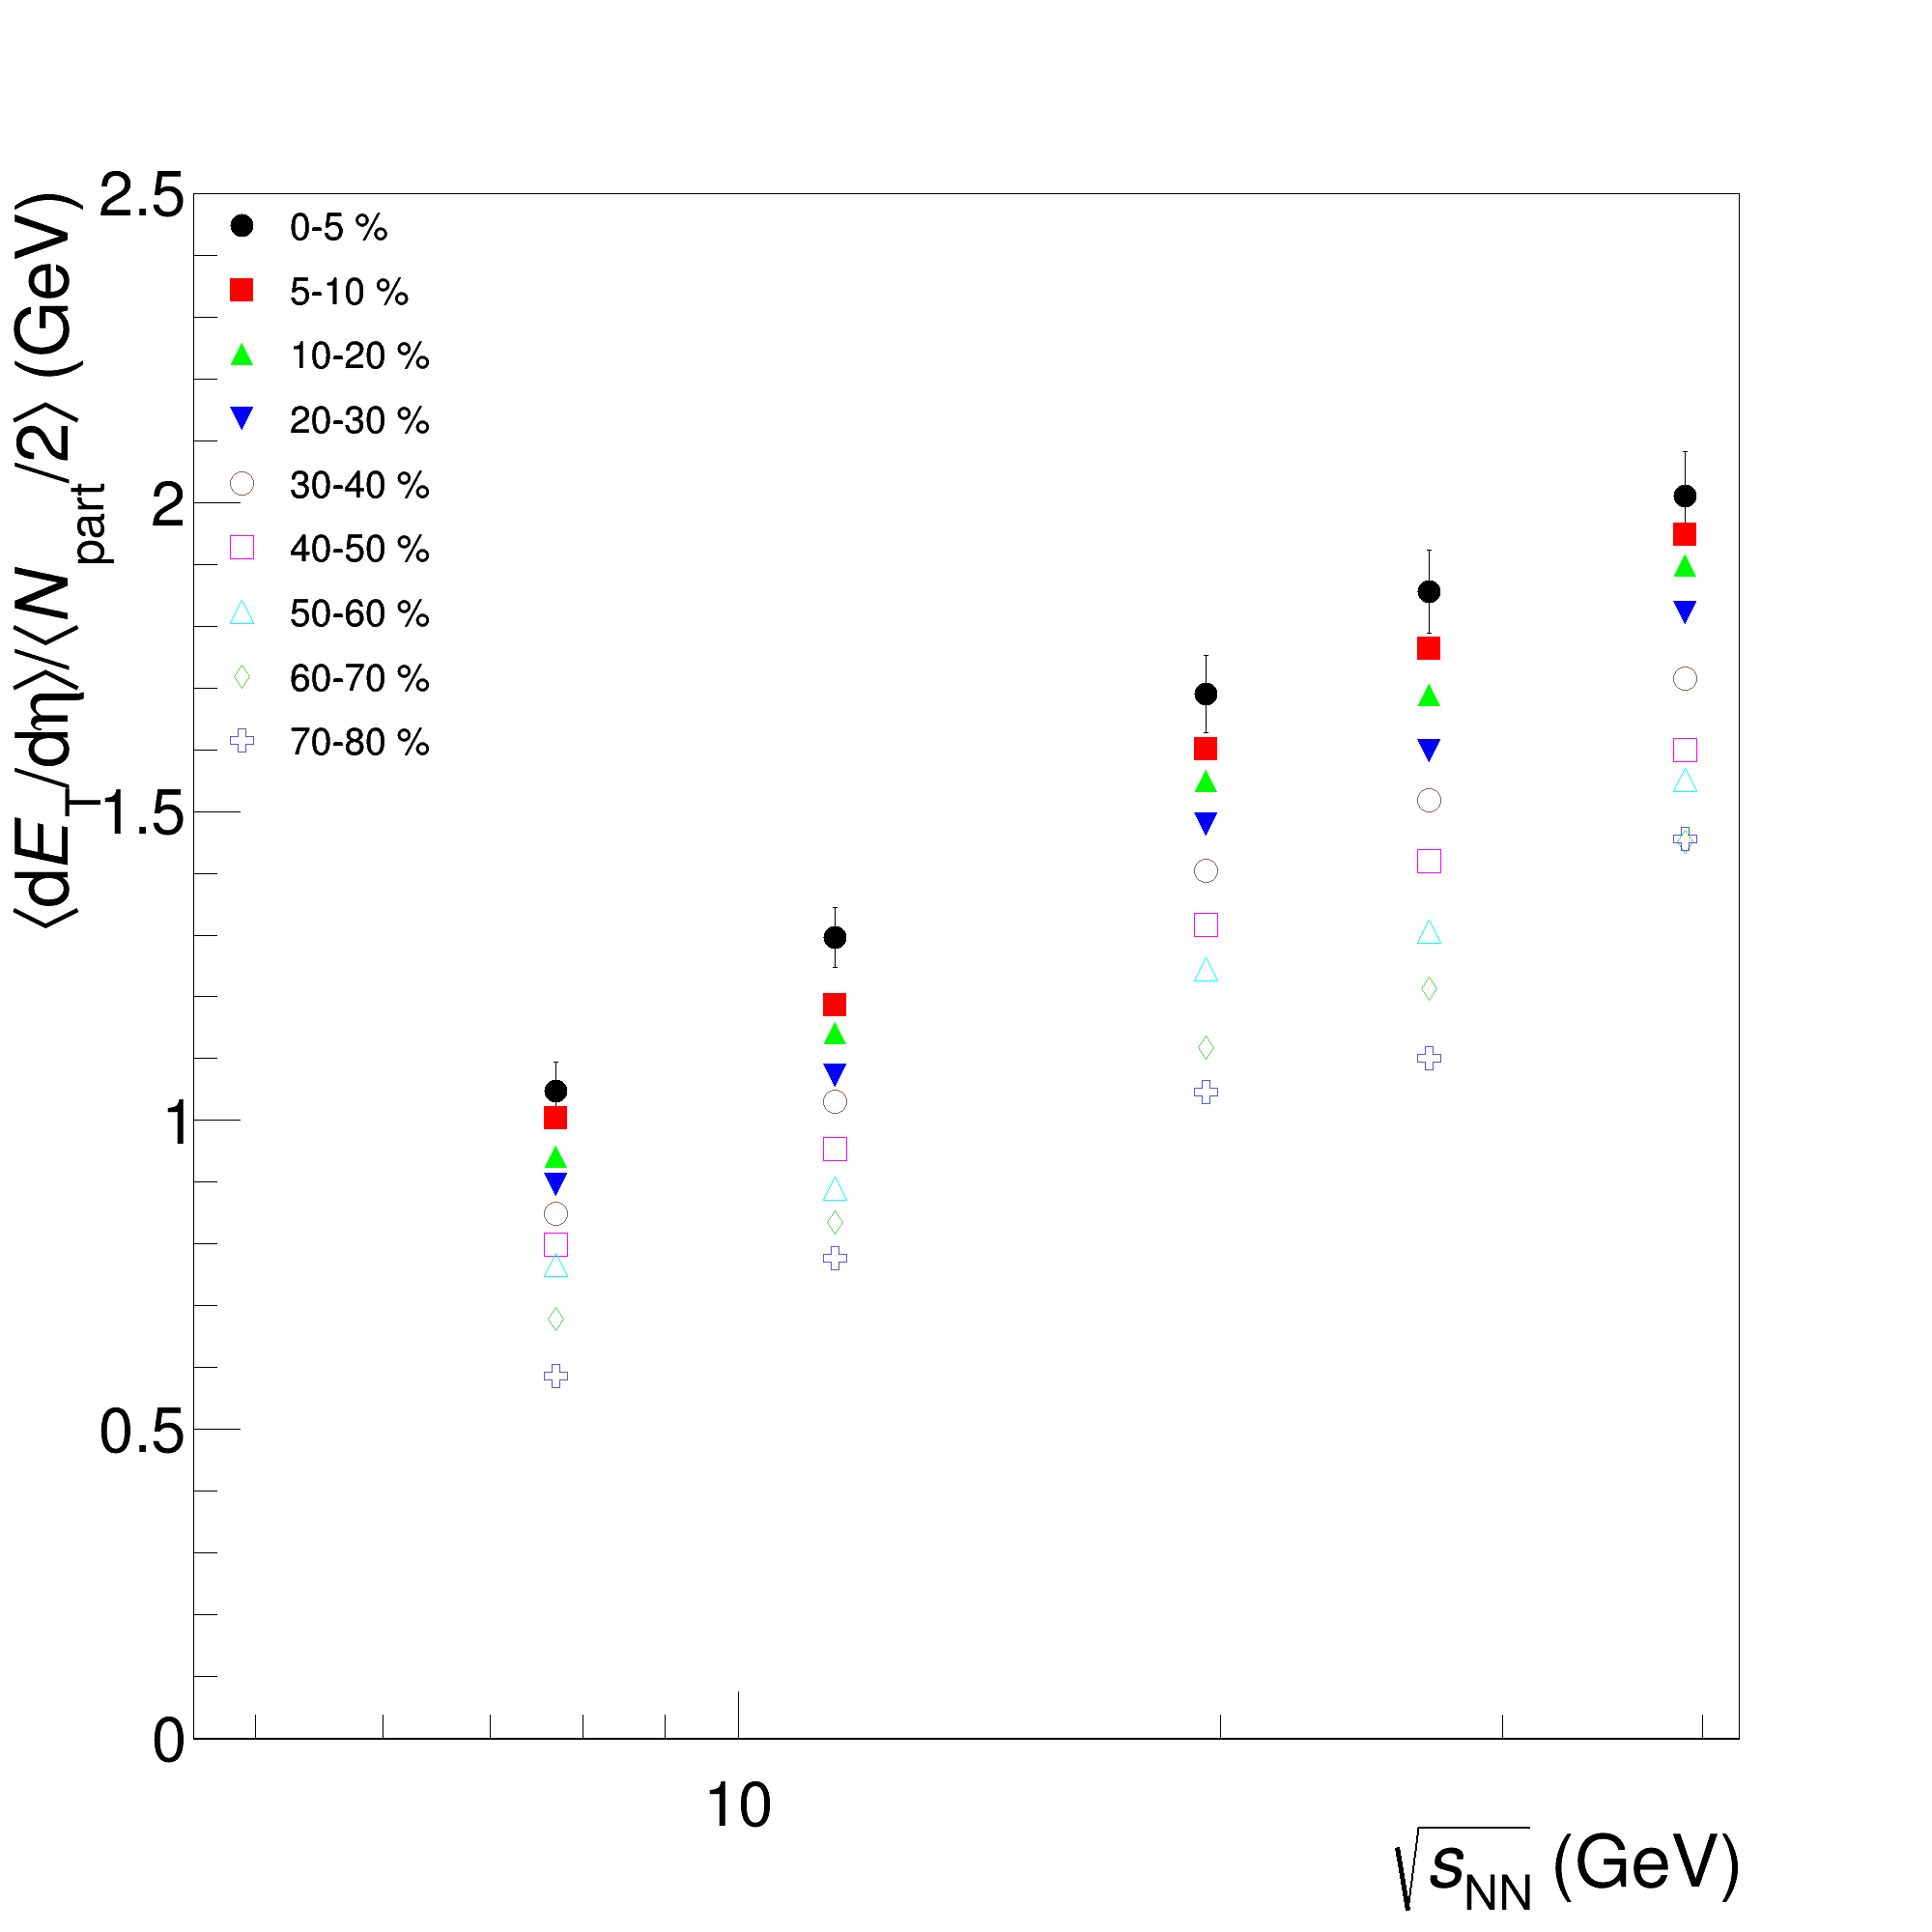
\includegraphics[width=5.5in]{figures/finalStacked/dETdEtaOverNpartBy2SumCent8s.png}
	  \caption{$(dE_{T}/d\eta)/0.5N_{part}$ at midrapidity as a function of $\sqrt{s_{NN}}$ for different centralities.}\label{fig:dETdEtaOverNpartBy2SumCents}
	\end{figure}
	
	\begin{figure}[h]
	  \centering
	  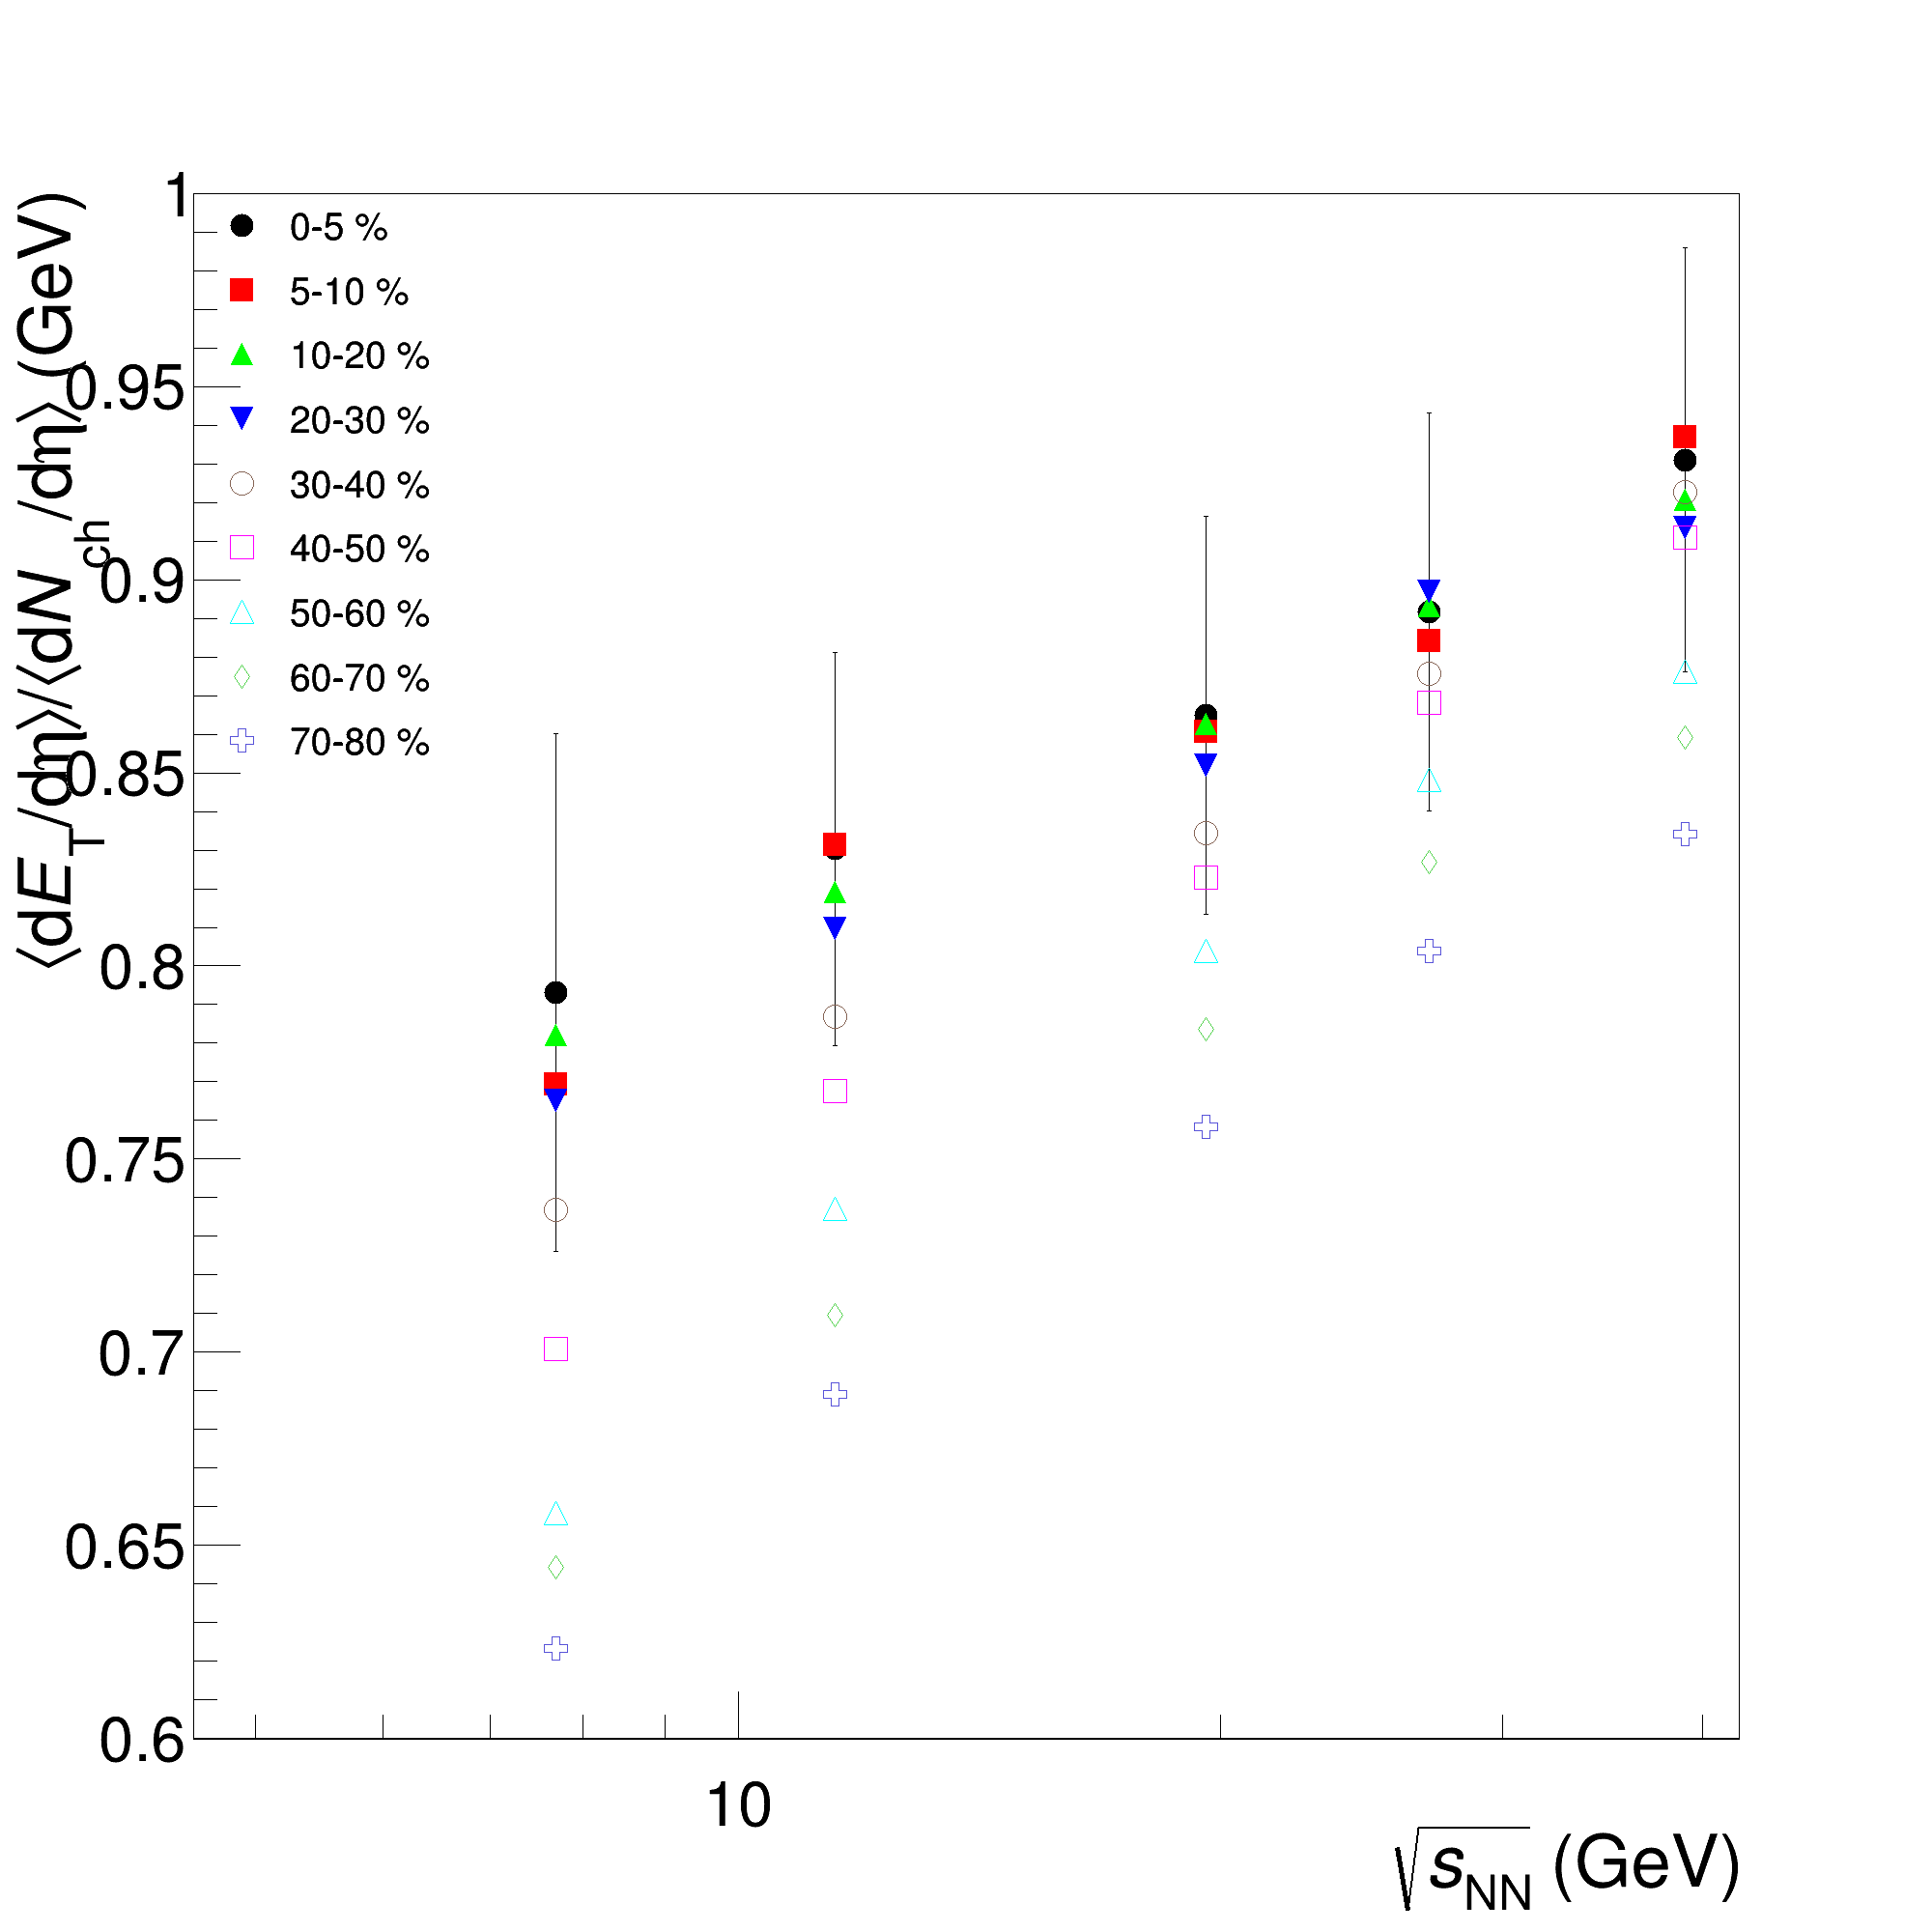
\includegraphics[width=5.5in]{figures/finalStacked/dETdEtaOverdNchdEtaSumCent8s.png}
	  \caption{$(dE_{T}/d\eta)/(dN_{ch}/d\eta)$ at midrapidity as a function of $\sqrt{s_{NN}}$ for different centralities.}\label{fig:dETdEtaOverdNchdEtaSumCents}
	\end{figure}
%cnt97kx Send this link to your invitees ... http://whenisgood.net/fndqz2a This is where your results will appear ... http://whenisgood.net/fndqz2a/results/cnt97kx And use this link to edit your event ... http://whenisgood.net/fndqz2a/edit/cnt97kx
